\documentclass{article}

\usepackage[utf8]{inputenc}
\usepackage{graphicx}
\usepackage{booktabs}
\usepackage{subcaption}
\usepackage{hyperref}

\title{A simple GPU ray tracer: Project report DD2360}
\author{Jacob Wahlgren \texttt{<jacobwah@kth.se>} \\ Expected grade: A}

\begin{document}

\maketitle

\section{Introduction}
% Background on the problem

Ray tracing is a 3D rendering technique enabling realistic optical effects by
simulating light rays. It is often used for visual effects and animation in film
and television. Using ray tracing is computationally expensive since a ray has
to be simulated for each pixel. However, since the rays are independent the
problem is embarrassingly parallel and easy to accelerate using GPUs.

\section{Methodology}
% Explain implementation

We used the Blinn-Phong shading model to render a scene with a single light source
and a single solid sphere. The image is written to a file in the PPM
format using 3 bytes per pixel. Each pixel is computed by one GPU thread in
square tile blocks of configurable size.

Since the task is IO bound, we investigate three different techniques for
writing the image to file. The \textbf{fwrite} version is the simplest, where
the whole image is rendered, then copied to RAM, and then written to file with a
single write call. The \textbf{mmap} version truncates the file to the output
size and then memory maps the whole file. Once the image is rendered it is
copied directly into the memory mapped file. The \textbf{streams} version uses
multiple overlapping streams to render, copy, and write chunks of the image in
parallel.

The code is available at \url{https://github.com/jacwah/cuda-raytracer}.

\section{Experimental setup}
% Gpu platform, software and hardware, tools

Experiments are run on the Tegner cluster at the PDC Center for High Performance
Computing at KTH. These nodes have two 12 core Intel E5-2690v3 Haswell
processors with 512 GB RAM. The performance is evaluated both on nodes with
NVIDIA Quadro K420 and the NVIDIA Tesla K80. The GPUs are programmed using CUDA.

The reference CPU implementation in Python was modified to call \verb|savefig|
to write the image to a file instead of displaying it interactively.

\section{Results}
% Validation, performance

Visual inspection of the generated images using the \verb|display| command
validated the results. Example images are shown in figure \ref{fig:output}.

The performance comparison of the CPU and GPU versions showed that the GPU
vastly outperforms the CPU version on this task. The difference was more
noticeable at larger image dimensions. In fact, results were not obtained for
the CPU version above image dimension 1000 since it was too slow. The results
are presented in figure \ref{fig:cpu}, were the Quadra K240 fwrite 8x8
configuration is used to represent the GPU.

We evaluate the performance of different GPU configurations at image size
1000x1000 (normal) and 100000x100000 (huge). The image files are 2.9 MB and 28
GB respectively. At the normal image size, all
configurations perform similarly to each other. The K240 is surprisingly
consistently faster.

\begin{figure}
    \begin{subfigure}{0.5\linewidth}
        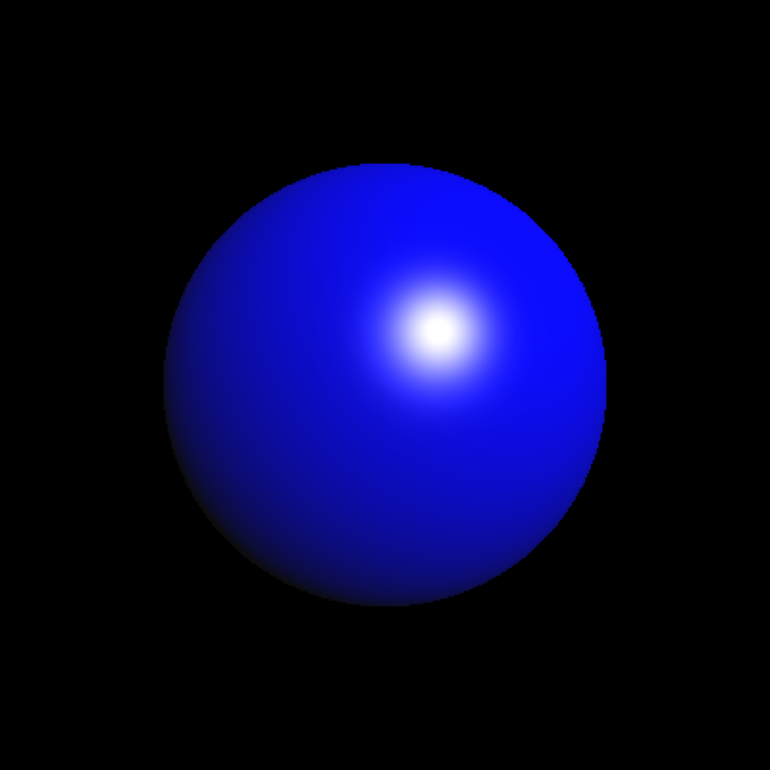
\includegraphics[width=\linewidth]{../raytracing_py_trim.png}
        \caption{CPU}
    \end{subfigure}
    \begin{subfigure}{0.5\linewidth}
        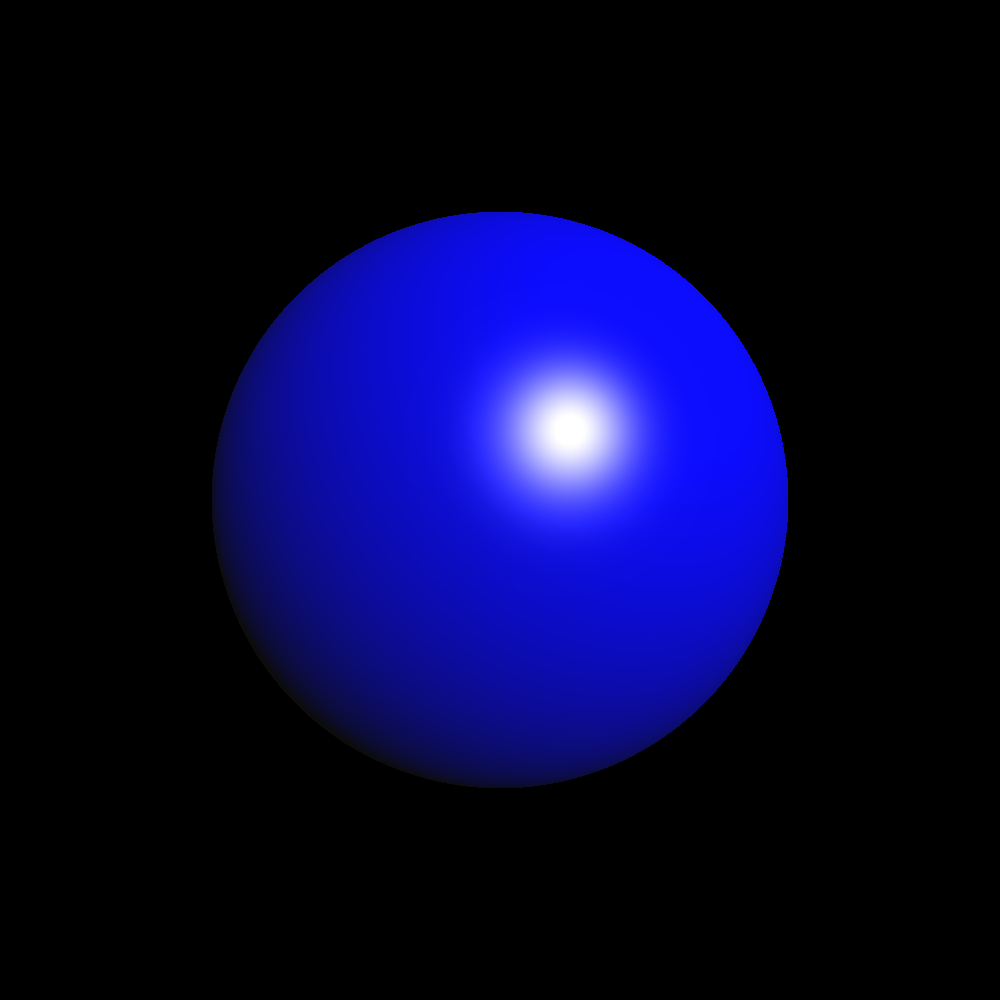
\includegraphics[width=\linewidth]{output.png}
        \caption{GPU}
    \end{subfigure}
    \caption{Sample output images.}
    \label{fig:output}
\end{figure}

\begin{figure}
    \centering
    \includegraphics{../fig/cpu.pdf}
    \caption{Performance comparison between Python CPU version and fwrite 8x8
    GPU version, average of 10 runs. Both run on Tegner thin nodes.}
    \label{fig:cpu}
\end{figure}

\begin{figure}
    \begin{subfigure}{\linewidth}
        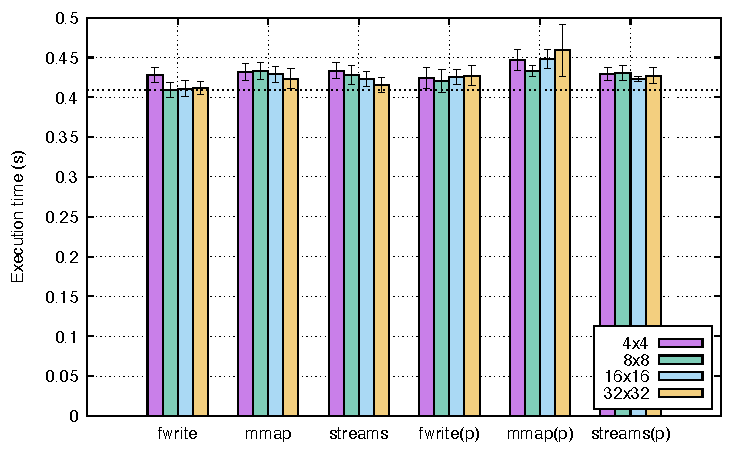
\includegraphics{../fig/sm30-1000.pdf}
        \caption{NVIDIA Quadro K240}
    \end{subfigure}
    \begin{subfigure}{\linewidth}
        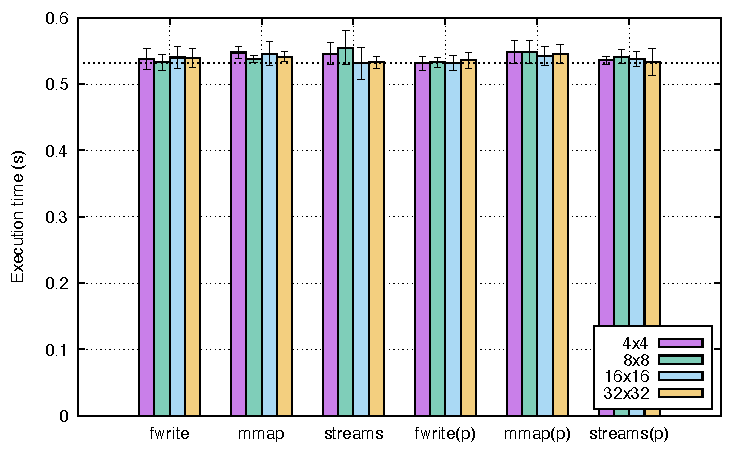
\includegraphics{../fig/sm37-1000.pdf}
        \caption{NVIDIA Tesla K80}
    \end{subfigure}
    \caption{Performance results for 1000x1000 image with various block sizes. Bars show average, whiskers show
    standard deviation.}
\end{figure}

\begin{figure}
    \begin{subfigure}{\linewidth}
        \includegraphics{../fig/sm30-100000.pdf}
        \caption{NVIDIA Quadro K240}
    \end{subfigure}
    \begin{subfigure}{\linewidth}
        %\includegraphics{../fig/sm37-100000.pdf}
        \caption{NVIDIA Tesla K80}
    \end{subfigure}
    \caption{Performance results for 100000x100000 image with various block
        sizes. Bars show average, whiskers show
    standard deviation.}
\end{figure}

\section{Discussion and conclusion}
% Discuss performance results
% Challenges and limitations
% Optimizations

The massive parallelism offered by the GPU vastly outperforms the reference CPU
implementation. However, a more fair comparison would use a faster language than
Python and utilize all the available compute power of the CPU rather than a
single thread.

The specular highlight in output images from the CPU and the GPU versions are
slightly different. This is likely caused by using different floating
point precision (double in Python, single in CUDA).

\end{document}
